\documentclass[12pt]{report}
\usepackage{xcolor, colortbl}
\usepackage{algorithm}
\usepackage[noend]{algpseudocode}
\usepackage{textcomp}
\usepackage{listings}
\usepackage{hyperref}
\usepackage{alltt}
\usepackage{tikz}
\usepackage{framed}
\usepackage{mdframed}
\usepackage{marvosym}
\usepackage{wasysym}
\usepackage{marvosym}
\usepackage{crayola}
\usepackage{mathpartir}
\usepackage{tabularx}
\usepackage[belowskip=-15pt,aboveskip=0pt]{caption}
\usepackage[skins]{tcolorbox}
\usepackage{multicol}
\usetikzlibrary{positioning,shapes,arrows, backgrounds, fit, shadows}
\usetikzlibrary{decorations.markings}
\usepackage{listings}
\usepackage[margin=1in]{geometry}
%\usepackage{mathptmx}
\usepackage{setspace}
\usepackage{natbib}
\usepackage{authblk}

\newcommand{\myheader}[1]{
	{\color{darkblue}
		\begin{Large}
			\begin{center}
				{#1}
			\end{center}
		\end{Large}
	}
}
\newcommand{\myminorheader}[1]{
	{\color{BrickRed}
		\begin{Large}
			{\fontfamily{\sfdefault}\selectfont\textbf{#1}}
		\end{Large}
	}
}

%\tikzstyle{input} = [coordinate]
%\tikzstyle{output} = [coordinate]


\tikzstyle{bb}=[%
      rectangle, draw=black, thick, fill=OliveGreen!30, drop shadow, align=center,
      text ragged, minimum height=2em, minimum width=2em, inner sep=6pt
]

\tikzstyle{inv}=[%
      rectangle, draw=none,  align=center,
      text ragged, minimum height=2em, minimum width=2em, inner sep=6pt
]

\tikzstyle{db}=[%
      ellipse, draw=black, thick, fill=pink, drop shadow, align=center,
      text ragged, minimum height=2em, inner sep=6pt
]

\tikzstyle{jn}=[%
      ellipse, draw=black, thick, fill=black, inner sep=0, outer sep=0,
]

\tikzstyle{io}=[%
      trapezium, trapezium left angle=60, trapezium right angle=120, draw=black, thick, fill=brown, drop shadow,
      text ragged, minimum height=2em, minimum width=2em, inner sep=6pt, align=center
]

\tikzstyle{glio}=[%
      trapezium, trapezium left angle=60, trapezium right angle=120, draw=red, line width = 1mm, fill=brown, drop shadow,
      text ragged, minimum height=2em, minimum width=2em, inner sep=6pt
]
\tikzstyle{gl}=[%
      rectangle, draw=red, line width = 1mm, fill=lightblue, drop shadow,
      text ragged, minimum height=2em, minimum width=2em, inner sep=6pt
]

\tikzstyle{en}=[%
      rectangle, draw=black, thick, fill=none,
      text ragged, minimum height=2em, minimum width=2em, inner sep=6pt
]

\tikzstyle{sh}=[%
      rectangle, draw=gray, thick, fill=none, color = gray,
      text ragged, minimum height=2em, minimum width=2em, inner sep=6pt
]


\lstdefinestyle{pc}{
	language = Python,
	basicstyle = \small\ttfamily,
	stringstyle = \ttfamily\color{Purple},
	keywordstyle=\color{black}\bfseries,
	identifierstyle=\ttfamily\color{BrickRed},
	frame=single,
	frameround=tttt,
	numbers=none,
	showstringspaces=false
}

\lstdefinestyle{cppc}{
	language = C++,
	basicstyle = \ttfamily\small,
	stringstyle = \color{red}\ttfamily,
	keywordstyle=\color{Blue}\bfseries,
	identifierstyle=\ttfamily,
	frame=single,
	frameround=tttt,
	numbers=none,
	showstringspaces=false,
	mathescape=true,
	escapeinside={(*@}{@*)}
}

\lstdefinestyle{occ}{
	language = Caml,
	basicstyle = \ttfamily,
	stringstyle = \color{red}\ttfamily,
	keywordstyle=\color{Blue}\bfseries,
	identifierstyle=\ttfamily,
	frameround=tttt,
	numbers=none,
	showstringspaces=false,
	escapeinside={(*@}{@*)}
}

\lstdefinestyle{oc}{
	language = bash,
	backgroundcolor = \color{black!60},
	basicstyle = \ttfamily\color{white},
	stringstyle = \color{red}\ttfamily,
	keywordstyle=\color{white}\bfseries,
	identifierstyle=\ttfamily,
	frameround=tttt,
	numbers=none,
	showstringspaces=false,
	escapeinside={(*@}{@*)}
}

\newcommand{\myslide}[1]{
\textbf{Slide:} \\
	\begin{framed}
			{#1}
	\end{framed}
}

\newcommand{\mynote}[1]{
\vspace{1cm}
\textbf{Note:} \\
	\fbox{
		\parbox{\textwidth}{%
			\colorbox{green!25}{
				\begin{minipage}{\textwidth}
					{#1}
				\end{minipage}
			}
		}
	}
}

\title{A System for Automated Evaluation of Objective Questions}
\begin{document}


\chapter{User Manual}
This software supports two types of objective question quizzes:
\begin{enumerate}
\item \textbf{Simple quiz:} In this quiz, the students are supposed to answer all questions.
\item \textbf{Jumbled quiz:} In this form of quiz, each student gets a different question paper to answer, which contains questions sampled out of a larger item bank.
\end{enumerate}

\section{Simple Quiz}

\begin{figure}[H]
\begin{center}
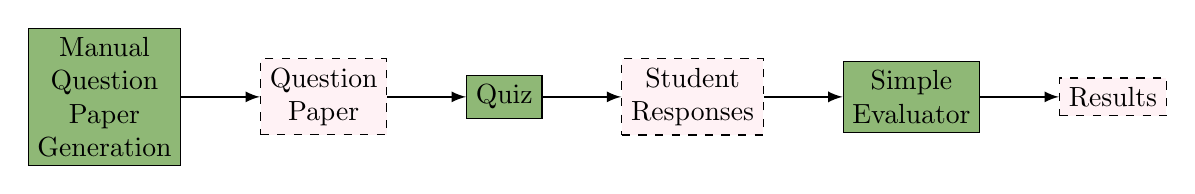
\begin{tikzpicture}
\node[draw=Black, fill=OliveGreen!50, align=center](qpgen){Manual \\ Question \\ Paper \\ Generation};
\node[dashed, draw=Black, fill=Pink!20, align=center, right=of qpgen](qp){Question \\ Paper};
\node[draw=Black, fill=OliveGreen!50, align=center, right=of qp](quiz){Quiz};
\node[dashed, draw=Black, fill=Pink!20, align=center, right=of quiz](sresp){Student \\ Responses};
\node[draw=Black, fill=OliveGreen!50, align=center, right=of sresp](seval){Simple \\ Evaluator};
\node[dashed, draw=Black, fill=Pink!20, align=center, right=of seval](res){Results};

\draw[-latex, thick] (qpgen) -- (qp);
\draw[-latex, thick] (qp) -- (quiz);
\draw[-latex, thick] (quiz) -- (sresp);
\draw[-latex, thick] (sresp) -- (seval);
\draw[-latex, thick] (seval) -- (res);

\end{tikzpicture}
\end{center}
\caption{Simple Quiz Workflow}
\label{f:squiz}
\end{figure}
The question paper creation for a simple quiz is manual. All students solve an identical question paper. The evaluation step directly runs on the student responses using the \lstinline[style=pc]@SimpleEvaluator@ module.

\section{Jumbled Quiz}
\begin{figure}[H]
\begin{center}
\resizebox{\textwidth}{!}{
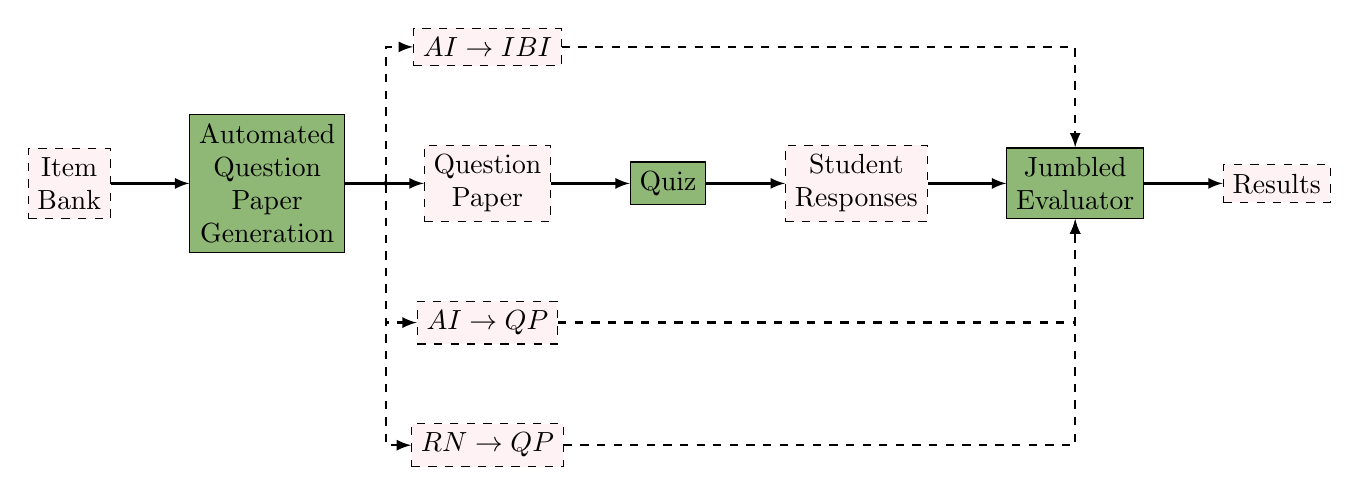
\begin{tikzpicture}
\node[dashed, draw=Black, fill=Pink!20, align=center](ib){Item \\ Bank};
\node[draw=Black, fill=OliveGreen!50, align=center, right=of ib](qpgen){Automated \\ Question \\ Paper \\ Generation};

\node[jn, right=0.5cm of qpgen](jn1) {};
\node[dashed, draw=Black, fill=Pink!20, align=center, right=of qpgen](qp){Question \\ Paper};
\node[dashed, draw=Black, fill=Pink!20, align=center, above=of qp](aiibi){$AI\rightarrow IBI$};
\node[dashed, draw=Black, fill=Pink!20, align=center, below=of qp](aiqp){$AI\rightarrow QP$};
\node[dashed, draw=Black, fill=Pink!20, align=center, below=of aiqp](rnqp){$RN\rightarrow QP$};

\node[draw=Black, fill=OliveGreen!50, align=center, right=of qp](quiz){Quiz};
\node[dashed, draw=Black, fill=Pink!20, align=center, right=of quiz](sresp){Student \\ Responses};
\node[draw=Black, fill=OliveGreen!50, align=center, right=of sresp](jeval){Jumbled \\ Evaluator};
\node[dashed, draw=Black, fill=Pink!20, align=center, right=of jeval](res){Results};

\draw[-latex, thick] (ib) -- (qpgen);
\draw[-, thick] (qpgen) -- (jn1);

\draw[-latex, thick] (jn1) -- (qp);
\draw[-latex, dashed, thick] (jn1) |- (aiibi);
\draw[-latex, dashed, thick] (jn1) |- (aiqp);
\draw[-latex, dashed, thick] (jn1) |- (rnqp);

\draw[-latex, thick] (qp) -- (quiz);
\draw[-latex, thick] (quiz) -- (sresp);
\draw[-latex, thick] (sresp) -- (jeval);
\draw[-latex, dashed, thick] (aiibi) -| (jeval);
\draw[-latex, dashed, thick] (aiqp) -| (jeval);
\draw[-latex, dashed, thick] (rnqp) -| (jeval);

\draw[-latex, thick] (jeval) -- (res);

\end{tikzpicture}
}
\end{center}
\caption{Jumbled Quiz Workflow}
\label{f:jquiz}
\end{figure}
The question paper creation step uses the \lstinline[style=pc]@genAIs@ (generate assessment items) and \lstinline@genQPs@ (generate question papers) modules. Once the question papers are generated, quiz is conducted. Finally, the automated evaluation process takes place using the \lstinline[style=pc]@JumbledEvaluator@ module.

\chapter{Design}
\section{Question Paper Codes}

\subsection{Question Paper Generation}
To discourage cheating in the class, we generate a set of question papers by randomly selecting $n$ questions out of an item-bank of $N$ questions. A set $K$ of distinct \emph{assessment instruments} are generated, numbered 0, 1, ..., $|K-1|$. We call them \emph{assessment instruments}.

The \emph{question paper generator} module $G$ generates a set $C$ of codes each of which can be mapped to any one of the assessment instruments of $K$. Each of the code $c$ in $C$ is finally mapped to one distinct question paper with $c$ printed on it. This way, the students will not be able to identify which assessment instrument $k \in K$ their copy of the question paper belongs to. Each question paper will have an empty table called the \emph{response table} on page one which will be used by the student to fill in his responses.

$G$ also generates a map from assessment instrument to question order. This tells us the original question number of each item in the give assessment instrument. For example:
\begin{figure}

\begin{center}
\begin{tabular}{|c|c|c|c|c|c|c|c|c|c|c|}
\hline
\cellcolor{Gray}0 & 3 & 5 & 1 & 4 & 9 & 12 & 15 & 2 & 10 & 2 \\
\hline
\cellcolor{Gray}1 & 4 & 1 & 2 & 11 & 6 & 7 & 5 & 14 & 8 & 12 \\
\hline
& \multicolumn{10}{|c|}{...} \\
\hline
\cellcolor{Gray}9 & 5 & 12 & 2 & 1 & 6 & 7 & 3 & 11 & 8 & 10 \\
\hline
\end{tabular}
\end{center}

\caption{Assessment Instrument Item to Item Bank Item map $AII \mapsto IBI$}
\label{f:aiiibi} 
\end{figure}

Figure~\ref{f:aiiibi} shows a possible mapping from assessment instruments to item bank items. The table can be interpreted as follows: There are 10 assessment instruments numbered 0 through 9. For each assessment instrument $AI \in K$ (here $|K| = 10$), there is a row in the table. Each cell in that row has the item bank item number for that item. For instance, for $AI = K[0]$, $AI[0] = 3$, $AI[1] = 5$ and so on.
  
This module will generate a map -- called $QP\mapsto AI$ between \emph{question paper code} to \emph{assessment instrument}. For example:

$QP\mapsto AI = [0, 1, 2, ..., 9, 0, 1, 2, ...]$ could be one such mapping. It says that $QP\mapsto AI[0] = 0$ (i.e. the question paper with code $0$ maps to assessment instrument number $0$). Similarly, $QP\mapsto AI[11] = 1$ (i.e. the question paper with code $11$ maps to assessment instrument number $1$) and so on.

\subsection{TA's Job}
The TA will note down following:
\begin{enumerate}
\item Question paper code for each roll number creating a \emph{roll number} to \emph{question paper code} map $RN\mapsto QP$.
\item transfer the responses into a CSV file corresponding to each student exactly as in the response table.
\end{enumerate}

\subsection{Automated Evaluation}
The \emph{response rearranger} refers to the $RN\mapsto QP$ and $QP\mapsto AI$ map to extract the assessment instrument for each roll number. Using this, the evaluator rearranges the responses in the order as per the item bank to create a rearranged response for the roll number $n$, $R'(n)$. This is given to the evaluator for final automated evaluation.
\end{document}
